\chapter{Modelos univariados para los pares de los contaminantes  $PM_{10}, PM_{2.5}$ y $O_3$}


\section{Correlación de dos procesos estocásticos}

En el presente capitulo se realizará la aplicación del modelo bivariado, haciendo uso de la función cópula construida para determinar el parámetro $\theta$ que describirá la correlación entre los dos procesos estocásticos en cuestión. Para este caso partícular se revisará de la siguiente manera: 
\begin{enumerate}
\item $PM_{10}$ vs $O_3$
\item $PM_{2.5}$ vs $O_3$
\item $PM_{10}$ vs $PM_{2.5}$
\end{enumerate}

Como primer paso se realizará una prueba que valide el funcionamiento correcto del modelo, para esto se realizará la simulación para el Ozono versus él mismo, para esto, se determinan los parámetros de las distribuciones a priori de la siguiente manera:Se retoma la información de la tabla \ref{infoestad} particularmente la media y la desviación estandar, con estos dos datos y sabiendo que para la distribución uniforme con parámetros $(a,b)$ se tiene: 

$$E(x)=\frac{(a+b)}{2}\hspace{2cm} Var(x)=\frac{(b-a)^2}{12} $$

De esta manera es inmediato identificar los valores de $a$ y $b$
$$1.21=\frac{(a+b)}{2}\hspace{2cm} (0.03)^2=\frac{(b-a)^2}{12} $$
Luego entonces, para el parámetro $\a$ los valores son $a=1.16$ y $b=1.26$, de manera análoga se realizan los cálculos para el parámetros $\b$ y también para los otros dos contaminantes. Al ejecutar el programa de computo se obtienen los siguientes resultados:


\begin{table}[!h]
\centering
\begin{tabular}{|l|l|l|l|l|l|}
\hline
& \multicolumn{5}{c|}{Información estadística $O_3$ vs $O_3$} \\
\cline{2-6}
Modelo & Parámetros & dist. inicial  & Media & sd  &   intervalo $95 \%$\\
\hline \hline
\multirow{5}{1.5cm}{Sin puntos de cambio } & $\theta$ & $unif(-1,1)$ & \textcolor{blue}{$0.9487761$} & $0.004088$ & $(0.8906871 ;0.9570268 )$ \\ \cline{2-6}
& $\a_1$& $unif(1.2,1.3)$ & $1.2000047$ & $0.0000497$ & $( 1.2000001;1.2000183)$\\  \cline{2-6}
& $\b_1$& $unif(10.9,15.8)$ & $13.3206233$ & $0.10380$ & $(13.1292662;13.5385384)$\\  \cline{2-6}
& $\a_2$& $unif(1.2,1.3)$ & $1.2000047$ & $0.0000465$ & $(1.2000001;1.2000163)$\\  \cline{2-6}
& $\b_2$& $unif(10.9,15.8)$ & $13.3157448$ & $0.10250$ & $(13.1135846;13.5139078)$\\  \cline{1-6}

\end{tabular}
\caption{Prueba del modelo bivariado}
\label{infoestad_prueba}
\end{table}

Como se puede observar en la tabla \ref{infoestad_prueba} el parámetro $\theta$ arroja un valor muy cercano a $1$ lo cual consistente y tiene sentido pues los datos estudiados son exactamente iguales, esta prueba genera confianza para poder determinar la correlación, ahora sí, entre cada par de contaminantes. 

\newpage
\subsection{Correlación, $\theta$, entre los contaminantes $PM_{10}$ y $O_3$ }

En esta sección se presentan los resultados obtenidos al ejecutar el modelo que relaciona el material particulado de 10 micras de tamaño, junto con el ozono. 

Como distribución a priori se elige, uniforme con parámetros $a,b$ y estos valores fueron encontrados tal como se mencionó anteriormente. La tabla \ref{infoestad_PM10_Oz} resume los resultados obtenidos para estos dos procesos estocásticos. 
\begin{table}[!h]
\centering
\begin{tabular}{|l|l|l|l|l|l|}
\hline
& \multicolumn{5}{c|}{Información estadística $PM_{10}$ y $O_3$ } \\
\cline{2-6}
Modelo & Parámetros & dist. inicial  & Media & sd  &   intervalo $95 \%$\\
\hline \hline
\multirow{5}{1.5cm}{Sin puntos de cambio }  & $\theta$ & $unif(-1,1)$ & $-0.9999994$ & $0.0000069$ & $(-1.0000000;-0.99999758 )$ \\ \cline{2-6}
& $\a_1$& $unif(0.803,0.977)$ & $0.8030031$ & $0.0002969$ & $( 0.8030001;0.8030110)$\\  \cline{2-6}
& $\b_1$& $unif(0.6,2.9)$ & $0.6000459$ & $0.000472$ & $(0.6000013;0.6001711)$\\  \cline{2-6}
& $\a_2$& $unif(1.2,1.3)$ & $1.2000027$ & $0.0000277$ & $(1.2000001;1.2000100)$\\  \cline{2-6}
& $\b_2$& $unif(10.9,15.8)$ & $15.4519679$ & $0.000493$ & $(15.3486982;15.5417151)$\\  \cline{1-6}
\end{tabular}
\caption{Correlación entre los contaminantes $PM_{10}$ y $O_3$  }
\label{infoestad_PM10_Oz}
\end{table}

Para este primer análisis, el resultado del parámetro $\theta$ arroja un resultado completamente correlacionado negativamente, pues su valor medio fue $-0.9999994$, esto lo que indica es que, con una alta probabilidad, el aumento de la contaminación de $PM_{10}$ afecta de manera inversa a la concentración de partículas de $O_3$ en el aire. 
Por otra parte en la tabla \ref{infoestad_PM10_Oz} se puede observar que el intervalo de confianza es reducido, esto se puede explicar, porque los parámetros de las distribuciones iniciales también lo son, principalmente los $\a_i$ de cada uno de los contaminantes. Para representar esta información de forma gráfica, se realizaron las curvas de nivel que se observan en la figura \ref{curv_niv_pm10_03}. En esta imagen, de color gris se representa la suma de los datos observados de $PM_{10}$ y $O_3$, las graficas de color verde y azul, representan el intervalo de confianza estimado para la función $m(t_1,t_2$ y la grafica de color verde, representa la estimación propuesta. Este análisis se realiza sin tener en cuenta algún punto de cambio, al igual que en el modelo univariado, si se empiezan a tener en cuenta, los resultados iran siendo óptimos en su proceso.

\begin{figure}[!h]
\begin{center}
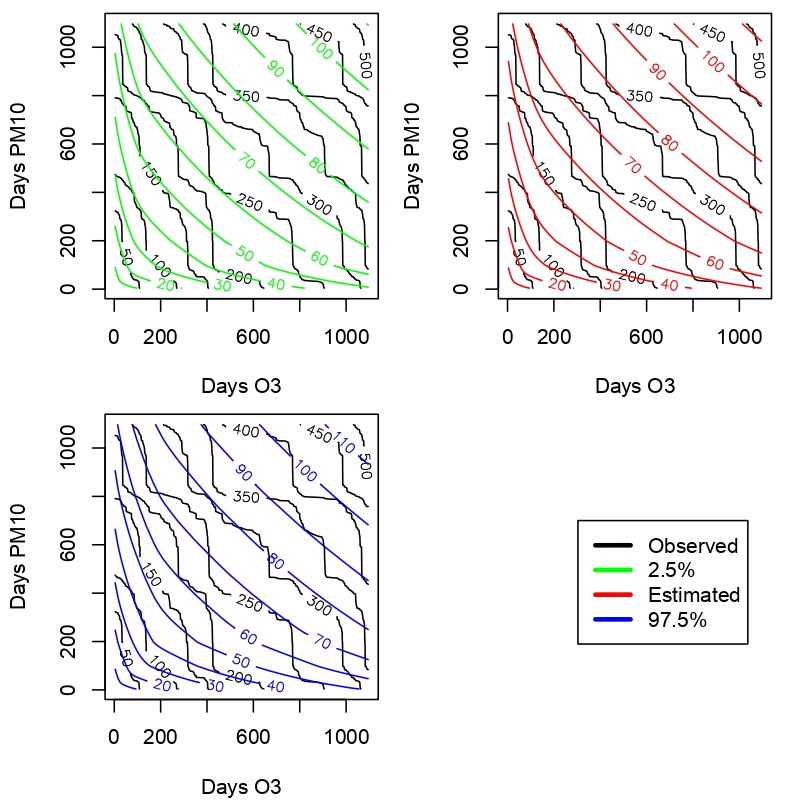
\includegraphics[scale=1]{cdnpm10vs03}
\end{center}
\centering
\caption{Curvas de nivel para los contaminantes $PM_{10}$ y $0_3$. \cite{EPA}}
\label{curv_niv_pm10_03}
\end{figure}


%%%%%%%%%%%%%%%%%%%%%%%%%%%%%%%%%%%%%%

\newpage
\subsection{Correlación, $\theta$, entre los contaminantes $PM_{2.5}$ y $O_3$ }

En la tabla \ref{infoestad_PM2.5_Oz}, se muestran los resultados obtenidos al ejecutar el código en R, se observa aquí algo interesante y es que la correlación es negativa y casi perfecta. Lo que quiere decir esto, es que a medida que los niveles de concentración de material partóculado de $2.5 \mu m$ de tamaño, los niveles de concentración de ozono disminuyen.

\begin{table}[!h]
\centering
\begin{tabular}{|l|l|l|l|l|l|}
\hline
& \multicolumn{5}{c|}{Información estadística $PM_{2.5}$ y $O_3$} \\
\cline{2-6}
Modelo & Parámetros & dist. inicial  & Media & sd  &   intervalo $95 \%$\\
\hline \hline
\multirow{5}{1.5cm}{Sin puntos de cambio } & $\theta$ & $unif(-1,1)$ & $-0.9999321$ & $0.000678$ & $(-0.9999980 ;-0.9997630 )$ \\ \cline{2-6}
& $\a_1$& $unif(1.2,1.3)$ & $0.7645434$ & $0.0000206$ & $( 0.7596495;0.7696293)$\\  \cline{2-6}
& $\b_1$& $unif(10.9,15.8)$ & $5.0000769$ & $0.00808$ & $(5.0000019;5.0002863)$\\  \cline{2-6}
& $\a_2$& $unif(1.2,1.3)$ & $0.6867448$ & $0.0000248$ & $(0.6820837;0.6916936)$\\  \cline{2-6}
& $\b_2$& $unif(10.9,15.8)$ & $5.0000812$ & $0.00808$ & $(5.0000025;5.0003026)$\\  \cline{1-6}

\end{tabular}
\caption{Correlación entre los contaminantes $PM_{10}$ y $O_3$  }
\label{infoestad_PM2.5_Oz}
\end{table}
\newpage

Al igual que en el caso anterior, a la información contenida en la tabla \ref{infoestad_PM2.5_Oz} se le realizó la respectiva representación por medio de curvas de nivel, essta información se puede observar en la figura \ref{curv_niv_pm25_03}, en ella se puede observar el ajuste del modelo, similar a como ocurria en el modelo univariado, donde los datos se ajustaban de buena manera, en el inicio de los días analizados, pero que luego, por los puntos de cambio el modelo se aleja un poco.


\begin{figure}[!h]
\begin{center}
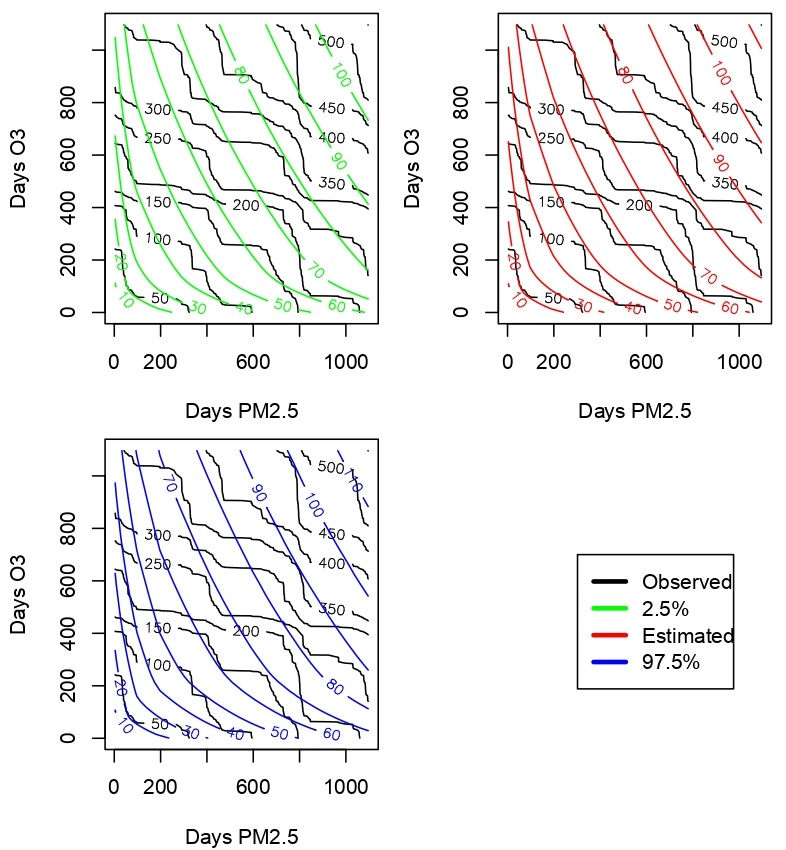
\includegraphics[scale=1]{cdn_ozpm25}
\end{center}
\centering
\caption{Curvas de nivel para los contaminantes $PM_{2.5}$ y $0_3$. \cite{EPA}}
\label{curv_niv_pm25_03}
\end{figure}


\subsection{Correlación, $\theta$, entre los contaminantes $PM_{2.5}$ y $PM_{10}$ }

El material particulado dentro del análisis presenta justo lo que se espera, pues por tratarse del mismo contaminante pero con distinto tamaño, se espera que los resultados de uno, de alguna manera, estan contenidos dentro del otro, esto significa que su correlación debe ser positiva y cercana a 1, y es justo lo que se puede observar en la tabla \ref{infoestad_PM10_PM2.5} donde el valor $\theta$ dio un resultado de $0.7546785$, esto continua resultados interesantes dentro del estudio porque concuerda con lo esperado.
 
\begin{table}[!h]
\centering
\begin{tabular}{|l|l|l|l|l|l|}
\hline
& \multicolumn{5}{c|}{Información estadística $PM_{2.5}$ y $PM_{10}$ } \\
\cline{2-6}
Modelo & Parámetros & dist. inicial  & Media & sd  &   intervalo $95 \%$\\
\hline \hline
\multirow{5}{1.5cm}{Sin puntos de cambio }
 & $\theta$ & $unif(-1,1)$ & $0.7546785$ & $0.008007$ & $(0.7390866;0.7693154 )$ \\ \cline{2-6}
& $\a_1$& $unif(1,3)$ & $1.0000078$ & $0.000789$ & $(1.0000002; 1.0000301)$\\  \cline{2-6}
& $\b_1$& $unif(7,20)$ & $8.0001299$ & $0.000129$ & $(8.0000029;8.0004811 )$\\  \cline{2-6}
& $\a_2$& $unif(1,3)$ & $1.0000105$ & $0.0000981$ & $(1.0000003; 1.0000364)$\\  \cline{2-6}
& $\b_2$& $unif(7,20)$ & $8.0001377$ & $0.0001347$ & $(8.0000046;8.0005117)$\\  \cline{1-6}

\end{tabular}
\caption{Correlación entre los contaminantes $PM_{10}$ y $PM_{2.5}$  }
\label{infoestad_PM10_PM2.5}
\end{table}

Para este par de contaminantes también se construyeron las curvas de nivel, figura \ref{curv_niv_pm10_pm25}, que asocian estos resultados. 
En este caso el modelo se ajusta de manera adecuada y de forma similar a los pares estudiados anteriormente, se pueden construir los modelos teniendo en cuenta algunos puntos de cambio en común para obtener un ajuste óptimo. 

\begin{figure}[!h]
\begin{center}
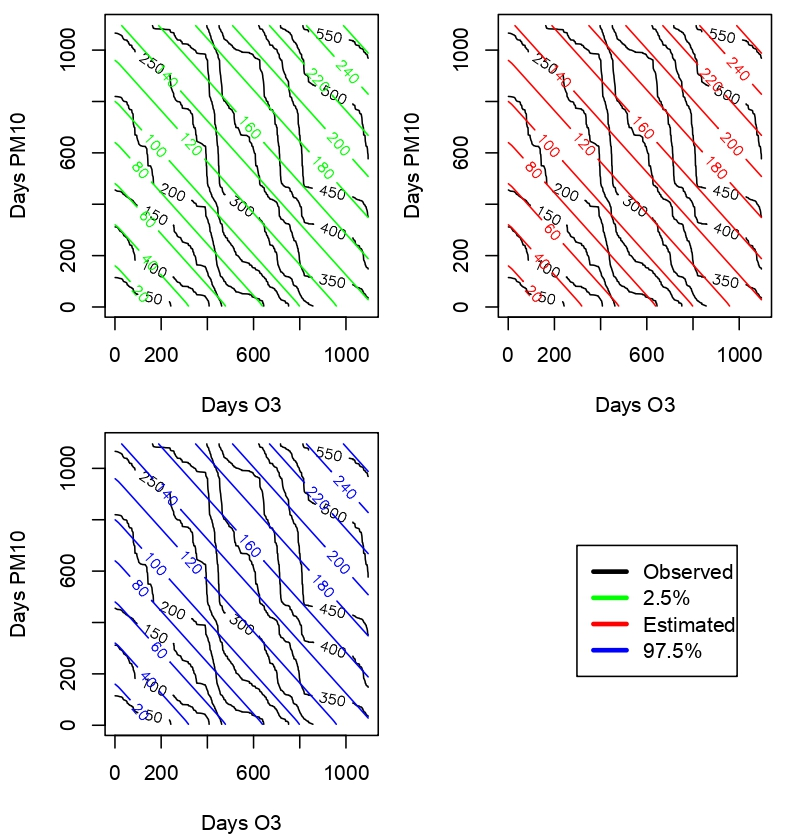
\includegraphics[scale=1]{cdnpm10vspm25}
\end{center}
\centering
\caption{Curvas de nivel para los contaminantes $PM_{10}$ y $PM_{2.5}$. }
\label{curv_niv_pm10_pm25}
\end{figure}